%!TEX root = main.tex

\section{Application Fields and Performance}

\begin{frame}{Application Fields and Performance}{Bechmark Problems}
  \begin{columns}
    \begin{column}[t]{0.575\textwidth}
      \textbf{Multi-body dynamics}
      \begin{enumerate}\small
        \setlength{\itemsep}{0.0em}
        \item Car-axis (index-3)
        \item Flexible slider-crank (index-3)
        \item Double-wishbone suspension (index-3)
      \end{enumerate}
      \textbf{Trajectory prescribed path control problems}
      \begin{enumerate}\setcounter{enumi}{3}\small
        \setlength{\itemsep}{0.0em}
        \item Space shuttle initial stage reentry (index-3)
        \item Space shuttle final stage reentry (index-2)
        \item Robotic arm control  (index-5)
      \end{enumerate}
    \end{column}
    \hspace{-0.055\textwidth}
    \begin{column}[t]{0.55\textwidth}
      \textbf{Electric circuits}
      \begin{enumerate}\setcounter{enumi}{6}\small
        \setlength{\itemsep}{0.0em}
        \item Eight-nodes transistor-amplifier (index-3)
        \item Electric ring modulator (index-1)
        \item Cascaded differential amplifiers (up to index-100)
      \end{enumerate}
      \textbf{Generic \acs{DAE} systems}
      \begin{enumerate}\setcounter{enumi}{9}\small
        \setlength{\itemsep}{0.0em}
        \item Particle motion (index-3);
        \item $2$-pendula (index-3)
        \item $3$-pendula (index-5)
        \item $4$-pendula (index-9)
        \item $5$-pendula (index-11)
      \end{enumerate}
    \end{column}
  \end{columns}
  \vspace{1.0em}
  \scriptsize{Most of the problems are taken from: \\
  \fullcite{mazzia2008test} \\
  \fullcite{brenan1995numerical}}
\end{frame}


\begin{frame}{Application Fields and Performance}{Benchmarking the Index Reduction Algorithm}
  \vspace{-1.0em}
  \begin{columns}
    \begin{column}[t]{0.5\textwidth}
      The \textbf{rules}
      \begin{itemize}\small
        \setlength{\itemsep}{0.0em}
        \item[\raisebox{-1pt}{\scalebox{0.8}{\faHourglassHalf}\,}] \SI{100}{\second} time limit for symbolic simplification
        \item[\raisebox{-1pt}{\scalebox{0.8}{\faInfinity}}] unlimited time for numerical integration
        \item[\raisebox{-1pt}{\scalebox{0.8}{\faCheck}}] if you can integrate the problem, you win
      \end{itemize}
    \end{column}
    \begin{column}[t]{0.5\textwidth}
      The \textbf{competitors} \\
      \begin{itemize}\small
        \setlength{\itemsep}{0.0em}
        \item \Maple{} \texttt{dsolve} (undisclosed)
        \item \Matlab{} \texttt{reduceDAEIndex} (Pantelides)
        \item \Matlab{} \texttt{reduceDAEToODE} (Gaussian elim.)
        \item \Mathematica{} \texttt{NDSolve} (Pantelides)
        \item \hi{\Maple{} + \Matlab{} Proposed}
      \end{itemize}
    \end{column}
  \end{columns}
  \vspace{0.5em}%
  \centering{\small\begin{tabular}{lcccccccccccccc}
    \toprule
    \multirow{2.25}{*}{\textbf{Solver}} & \multicolumn{14}{c}{\textbf{Problems}} \\
    \cmidrule(l{4pt}r{4pt}){2-15}
    & 1 & 2 & 3 & 4 & 5 & 6 & 7 & 8 & 9 & 10 & 11 & 12 & 13 & 14 \\
    \midrule
    \rowcolor{mycolor2!25}
    \texttt{dsolve} & \mycheckmark & \mycheckmark & \mycrossmark & \mycheckmark & \mycrossmark & \mycrossmark & \mycrossmark & \mycheckmark & \mycrossmark & \mycrossmark & \mycrossmark & \mycheckmark\mywarnmark & \mycrossmark & \mycrossmark \\
    \rowcolor{mycolor3!25}
    \texttt{NDSolve} & \mycheckmark & \mycheckmark & -- & -- & -- & -- & -- & -- & -- & -- & \mycrossmark & \mycheckmark & -- & -- \\
    \rowcolor{mycolor3!25}
    \texttt{reduceDAEIndex} & \mycheckmark & \mycheckmark & -- & -- & -- & -- & -- & -- & -- & -- & \mycrossmark & \mycheckmark & -- & -- \\
    \rowcolor{mycolor3!25}
    \texttt{reduceDAEToODE} & \mycheckmark & \mycheckmark & -- & -- & -- & -- & -- & -- & -- & -- & \mycrossmark & \mycheckmark & -- & -- \\
    \rowcolor{mycolor5!25}
    \hi{Proposed} & \mycheckmark & \mycheckmark & \mycheckmark & \mycheckmark & \mycheckmark\mywarnmark & \mycheckmark\mywarnmark & \mycheckmark\mywarnmark & \mycheckmark & \mycheckmark & \mycheckmark & \mycrossmark & \mycheckmark & \mycheckmark & \mycheckmark \\
    \bottomrule
    \multicolumn{14}{l}{* Incomplete testing results.}
  \end{tabular}} \\[0.5em]
  \raggedright\scriptsize{\fullcite{schwarz2020singularities}}
\end{frame}

\begin{frame}{Application Fields and Performance}{Factorizations Performance}
  \vspace{-4.0em}
  \begin{columns}
    \centering
    \begin{column}[b]{0.525\textwidth}
      \hic{\acs{LU} performs better than \acs{FFLU}}
    \end{column}
    \begin{column}[b]{0.215\textwidth}
      \vspace{-1.0em}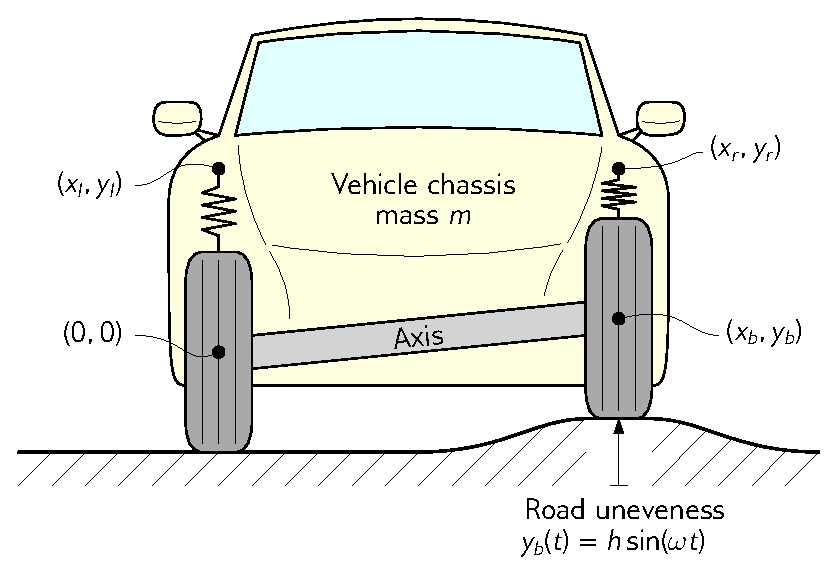
\includegraphics[width=\textwidth]{figures/car_axis.eps}
    \end{column}
  \end{columns}
  \centering{\scriptsize\begin{tabular}{cccc}
    \multicolumn{4}{c}{\textbf{Car-Axis (Index-3) -- \acs{LU} Factorization}} \\
    \toprule
    \textbf{Original \acsp{DAE}} & \multicolumn{3}{c}{$\mF = 108\cf + 131\cm + 56\ca$ \quad $\mh = 0$} \\
    \midrule
    \textbf{Reduction step} & $\mE$ & $\mg$ & $\ma$ \\
    \midrule
    Index-3 \acsp{DAE} & $12\cm$ & $94\cf + 145\cm + 54\ca$ & $14\cf + 16\cm + 10\ca$ \\
    Index-2 \acsp{DAE} & $12\cm$ & $94\cf + 145\cm + 54\ca$ & $26\cf + 45\cm + 15\ca$ \\
    Index-1 \acsp{DAE} & $12\cm$ & $94\cf + 145\cm + 54\ca$ & $136\cf + 4\cd + 261\cm + 95\ca$ \\
    Index-0 \acsp{DAE} & $1060\cf + 38\cd + 1901\cm + 717\ca$ & $431\cf + 8\cd + 842\cm + 268\ca$ & $0$ \\
    \midrule
    \rowcolor{mycolor5!25}
    \textbf{Reduced \acsp{DAE}} & \multicolumn{3}{c}{$\mF = 896\cf + 4\cd + 1202\cm + 546\ca$ \quad $\mh = 176\cf + 4\cd + 322\cm + 120\ca$} \\
    \bottomrule \\[0.05em]
    %
    \multicolumn{4}{c}{\textbf{Car-Axis (Index-3) -- \acs{FFLU} Factorization}} \\
    \toprule
    \textbf{Original \acsp{DAE}} & \multicolumn{3}{c}{$\mF = 108\cf + 131\cm + 56\ca$ \quad $\mh = 0$} \\
    \midrule
    \textbf{Reduction step} & $\mE$ & $\mg$ & $\ma$ \\
    \midrule
    Index-3 \acsp{DAE} & $0$ & $94\cf + 8\cd + 150\cm + 54\ca$ & $14\cf + 21\cm + 10\ca$ \\
    Index-2 \acsp{DAE} & $0$ & $94\cf + 8\cd + 154\cm + 54\ca$ & $26\cf + 1\cd + 44\cm + 15\ca$ \\
    Index-1 \acsp{DAE} & $0$ & $94\cf + 8\cd + 155\cm + 54\ca$ & $136\cf + 6\cd + 4\cd + 261\cm + 95\ca$ \\
    Index-0 \acsp{DAE} & $1066\cf + 55\cd + 1888\cm + 717\ca$ & $431\cf + 18\cd + 851\cm + 268\ca$ & $0$ \\
    \midrule
    \rowcolor{mycolor2!25}
    \textbf{Reduced \acsp{DAE}} & \multicolumn{3}{c}{$\mF = 1549\cf + 73\cd + 2765\cm + 1011\ca$ \quad $\mh = 176\cf + 7\cd + 326\cm + 120\ca$} \\
    \bottomrule
  \end{tabular}}
\end{frame}

\begin{frame}{Application Fields and Performance}{Expression Swell}
  \begin{columns}
    \centering
    \begin{column}[c]{0.7\textwidth}
      \hic{And when strong expression swell arise \dots}
    \end{column}
    \begin{column}[c]{0.22\textwidth}
      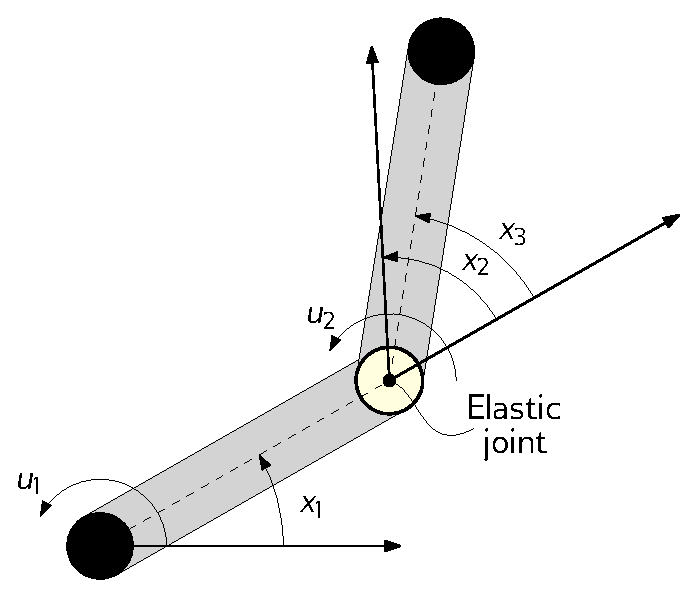
\includegraphics[width=\textwidth]{figures/robotic_arm.eps}
    \end{column}
  \end{columns}
  \hspace{-0.5em}
  \centering{\scriptsize\begin{tabular}{cccc}
    \multicolumn{4}{c}{\textbf{Robotic Arm (Index-5)}} \\
    \toprule
    \textbf{Original \acsp{DAE}} & \multicolumn{3}{c}{$\mF = 125\cf + 19\cd + 56\cm + 64\ca$ \quad $\mh = 0$} \\
    \midrule
    \textbf{Reduction step} & $\mE$ & $\mg$ & $\ma$ \\
    \midrule
    Index-5 \acsp{DAE} & $0$ & $66\cf + 3\cd + 50\cm + 35\ca$ & $16\cf + 12\ca$ \\
    Index-4 \acsp{DAE} & $0$ & $66\cf + 3\cd + 50\cm + 35\ca$ & $24\cf + 6\cm + 14\ca$ \\
    Index-3 \acsp{DAE} & $0$ & $66\cf + 3\cd + 50\cm + 35\ca$ & $162\cf + 2\cd + 138\cm + 114\ca$ \\
    Index-2 \acsp{DAE} & $14\cf + 2\cd + 6\cm + 6\ca$ & $372\cf + 4\cd + 375\cm + 253\ca$ & $972\cf + 1\cd + 1062\cm + 770\ca$ \\
    \rowcolor{mycolor2!25}
    Index-1 \acsp{DAE} & $14\cf + 2\cd + 6\cm + 6\ca$ & $372\cf + 4\cd + 375\cm + 253\ca$ & $\star (6.5\cf + 5.6\cm + 1.8\ca)\!\cdot\!10^{6} + 4\cd$ \\
    \rowcolor{mycolor2!25}
    Index-0 \acsp{DAE} & $\star (8.3\cf + 7.1\cm + 2.3\ca)\!\cdot\!10^{7} + 58\cd$ & $(2.4\cf + 2.0\cm + 0.9\ca)\!\cdot\!10^{6} + 8\cd$ & $0$ \\
    \midrule
    \rowcolor{mycolor2!25}
    \textbf{Reduced \acsp{DAE}} & \multicolumn{3}{c}{$\star \mF = (8.6\cf + 7.3\cm + 2.4\ca)\!\cdot\!10^{7} + 66\cd$ \quad $\star \mh = (6.5\cf + 5.6\cm + 1.8\ca)\!\cdot\!10^{6} + 7\cd$} \\
    \bottomrule
    \end{tabular}}
\end{frame}

\begin{frame}{Application Fields and Performance}{Expression Swell Mitigation}
  \vspace{-2.0em}
  \hic{\dots hierarchical representation does the job}
  \vspace{-0.5em}
  \centering{\scriptsize\begin{tabular}{cccc}
    \multicolumn{4}{c}{\textbf{Robotic Arm (Index-5)}} \\
    \toprule
    \textbf{Original \acsp{DAE}} & \multicolumn{3}{c}{$\mFv = 125\cf + 19\cd + 56\cm + 64\ca$ \quad $\mhv = 0$ \quad $\mv = 0$} \\
    \midrule
    \textbf{Reduction step} & $\mEv$ & $\mgv$ & $\mav$ \\
    \midrule
    Index-5 \acsp{DAE} & $0$ & $66\cf + 3\cd + 50\cm + 35\ca$ & $16\cf + 12\ca$ \\
    Index-4 \acsp{DAE} & $0$ & $66\cf + 3\cd + 50\cm + 35\ca$ & $24\cf + 6\cm + 14\ca$ \\
    Index-3 \acsp{DAE} & $0$ & $66\cf + 3\cd + 50\cm + 35\ca$ & $162\cf + 2\cd + 138\cm + 114\ca$ \\
    Index-2 \acsp{DAE} & $14\cf + 2\cd + 6\cm + 6\ca$ & $66\cf + 1\cv + 3\cd + 51\cm + 35\ca$ & $1\cm + 1\cv$ \\
    \rowcolor{mycolor5!25}
    Index-1 \acsp{DAE} & $2\cv + 1\ca$ & $66\cf + 1\cv + 3\cd + 51\cm + 35\ca$ & \cellcolor{mycolor5!25}$9\cf + 4\cv + 2\cd + 8\cm + 5\ca$ \\
    \rowcolor{mycolor5!25}
    Index-0 \acsp{DAE} & $7\cv + 1\cd + 2\cm + 2\ca$ & \cellcolor{mycolor5!25}$66\cf + 2\cv + 3\cd + 52\cm + 35\ca$ & $0$ \\
    \midrule
    \rowcolor{mycolor5!25}
    \textbf{Reduced \acsp{DAE}} & \multicolumn{3}{c}{$\mFv = 90\cf + 9\cv + 4\cd + 63\cm + 48\ca$ \quad $\mhv = 202\cf + 5\cv + 4\cd + 141\cm + 130\ca$} \\
    \bottomrule \\[-0.65em]
  \end{tabular}}
  \begin{columns}
    \centering
    \begin{column}[c]{0.5\textwidth}
      \centering{\scriptsize\begin{tabular}{cc}
        \multicolumn{2}{c}{Hierarchical representation details (29 veils)} \\
        \toprule
        \textbf{Reduction step} & $\mv$ \\
        \midrule
        Index-5 \acsp{DAE} & $0$ \\
        Index-4 \acsp{DAE} & $0$ \\
        Index-3 \acsp{DAE} & $0$ \\
        Index-2 \acsp{DAE} & $1278\cf + 3\cv + 6\cd + 1319\cm + 918\ca$ \\
        \rowcolor{mycolor3!25}
        Index-1 \acsp{DAE} & $8401\cf + 20\cv + 24\cd + 9451\cm + 6095\ca$ \\
        \rowcolor{mycolor3!25}
        Index-0 \acsp{DAE} & $37010\cf + 558\cv + 56\cd + 45087\cm + 28665\ca$ \\
        \midrule
        \rowcolor{mycolor3!25}
        \textbf{Reduced \acsp{DAE}} & $\mv = 37010\cf + 558\cv + 56\cd + 45087\cm + 28665\ca$ \\
        \bottomrule
      \end{tabular}}
    \end{column}
    \hspace{1.0em}
    \begin{column}[c]{0.215\textwidth}
      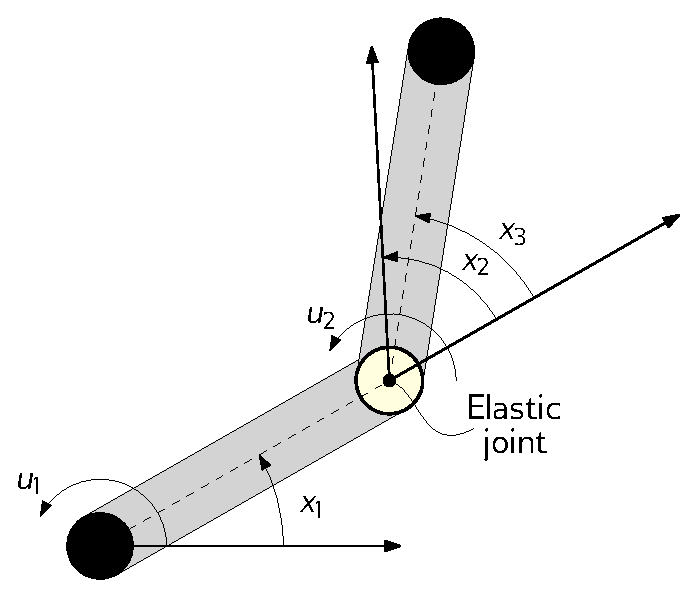
\includegraphics[width=\textwidth]{figures/robotic_arm.eps}
    \end{column}
  \end{columns}
\end{frame}

\begin{frame}{Application Fields and Performance}{Numerical Stability}
  \vspace{-2.0em}\begin{columns}
    \centering
    \begin{column}[c]{0.3\textwidth}
      \hic{Numerical\vphantom{y} stability is preserved but not guaranteed}
      \includegraphics[width=\textwidth]{figures/fade_overview.png}
    \end{column}
    \begin{column}[c]{0.7\textwidth}
      \vspace{1em}\small{\input{figures/suspension_pista_azzurra.tex}}
    \end{column}
  \end{columns}
\end{frame}

% That's all Folks!